\subsection{Project structure}

The implementation contains scripts, configuration file as well as folders containing data. Each script has defined a specific functionality and can be run by the command-line interface (CLI). The system has the following structure:

\begin{itemize}
    \item data/
    \item masterFrames/
    \item realData/
    \item config.yml
    \item windowCutter.py
    \item configuration.py
    \item starGen.py
\end{itemize}


\subsubsection{Folders}
Generated data are saved in the $data$ folder, where each series is saved in its own folder. Real DARK, BIAS, and FLAT FIELD frames are loaded from the folder $masterFrames$. And TSV files that are used for generating series from files are loaded from the folder $realData$. All these folders are not mandatory for the project and were only added based on our preference. The user can define the path to files and destination for generated data in the configuration $config.yml$. 

\subsubsection{Config.yml}
The configuration file is written in the YAML language. In the beginning, there are general settings, followed by a definition of each object and its parameters. All these settings were explained in the previous Section \ref{sec:sdgenerator}. An example of a defined object is shown in the Listing \ref{listing:yml}.

\begin{listing}[!ht]
\begin{minted}{yaml}
Objects:
  enable: True
  count:
    min: 1
    max: 5
    random: uniform
  brightness:
    min: 5000
    max: 20000
    random: uniform
  fwhm:
    min: 3.5
    max: 4
    random: uniform
\end{minted}
\caption{Structure of defined object in config.yml.}
\label{listing:yml}
\end{listing}


\subsubsection{windowCutter.py}
The script contains one class $Cutter$ and its only function is to cut windows of predefined size from input FITS images. The constructor of the class takes one argument that defines the desired size of the window. The $cut$ method first loads all FITS files contained in the defined path. Then slides the window over each image with a stride of half the size of the window. Cut images are then saved as FITS files in the defined destination folder. The script was implemented only for the purpose of cutting real DARK, BIAS, and FLAT FIELD frames into 50x50 cutouts needed for our training data. 

\subsubsection{configuration.py}
The goal of the script is to read and parse configuration file to Python classes, to be easily accessible during the generation process. The script contains multiple data classes as shown in the Figure  \ref{img:configurationClass}. Each object in the configuration file is encapsulated into its own Python class, which contains all the parameters as variables. All objects are then encapsulated into the $Configuration$ object, which also contains the values of the general settings of the system. There are also auxiliary classes $IntValue$ and $FloatValue$ that represent the range of number values and also provide a function to choose random values from the range. If the script is run directly by CLI it produces $Configuration$ object containing parsed data from $config.yml$.

\begin{figure}[h]
    \centering
    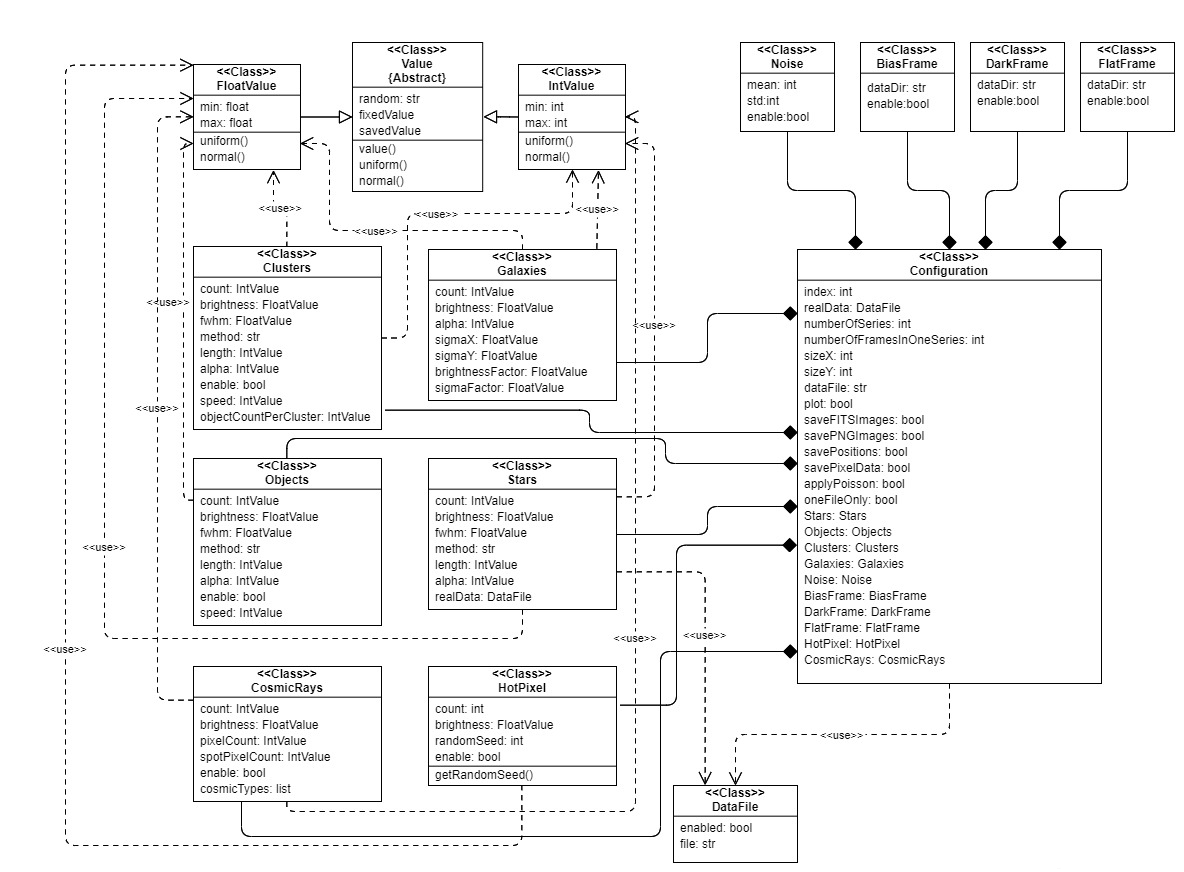
\includegraphics[width=.9\textwidth]{images/configuration.jpg}
    \caption{Class diagram of configuration.py script.}
    \label{img:configurationClass}
\end{figure}


\subsubsection{starGen.py}
At the core of the whole system is the $starGen.py$ script, whose goal is the generation of images. In the beginning, the script reads the $config.yml$ file using $configuration.py$ script. The output $Configuration$ object is then sent to the $StarGenerator$ class that generates a series of images. The script contains the following classes, which are also shown in the Figure \ref{img:starGenClass}:

\begin{itemize}
    \setlength\itemsep{1px}
    \item \textbf{StarGenerator} \\
    The main class that generates a series of images. The class receives the configuration data and generates astronomical objects based on the data specified by the user. With the help of other classes, it draws generated objects in the image, adds noises and defects, and saves the output files to a defined destination. 
    
    \item \textbf{DefectDrawingTool} \\
    The aim of the class is to add noises and defects to the generated image. It adds Gaussian noise, hot pixels, and cosmic rays as well as real DARK, BIAS, and FLAT FIELD frames to the image. 
    
    \item \textbf{DrawingTool} \\
    The class draws astronomical sources based on generated parameters onto the image. It supports the profile of streak and point source and elliptical galaxies. 
    
    \item \textbf{TSVSaver} \\ 
    The class is used for saving objects‘ positions in the TSV file.
    
    \item \textbf{ImageSaver} \\
    Saves the output images into FITS and PNG files. 
    
    \item \textbf{FileReader} \\
    Reads and parses TSV file that contains positions and brightness of stars and moving objects. 
    
    \item \textbf{FITSReader} \\
    Reads and loads real BIAS, DARK and FLAT FIELD FITS images. 
    
    \item \textbf{Utils} \\
    Contains a wide range of methods, that help with the drawing of objects, calculating positions or bounds, etc. 

\end{itemize}

\begin{figure}[H]
    \centering
    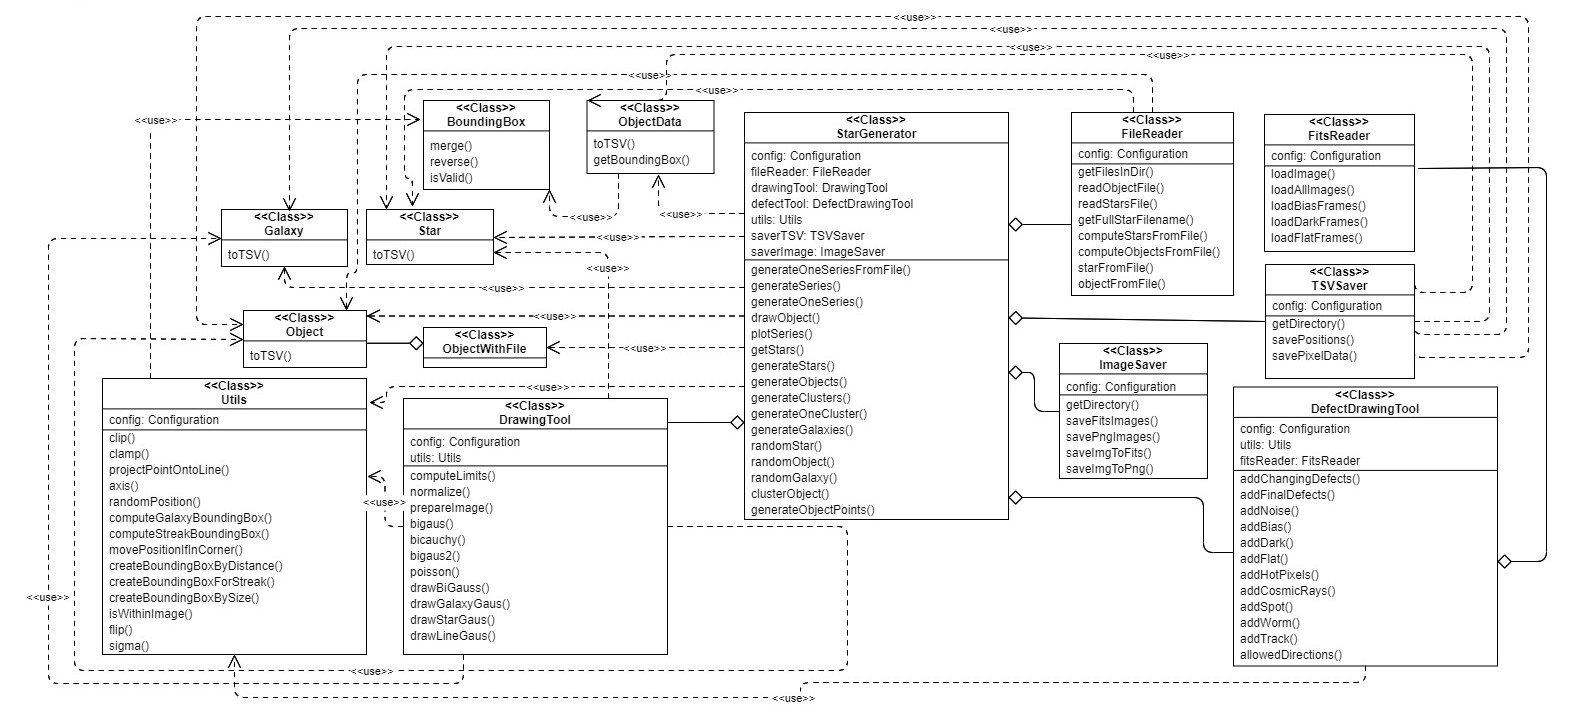
\includegraphics[width=\textwidth]{images/starGenClass3.jpg}
    \caption{Class diagram of starGen.py script.}
    \label{img:starGenClass}
\end{figure}


